\documentclass[11pt]{article}
\usepackage{amsmath}
\usepackage{amssymb}
\usepackage{caption}
\usepackage{subfig}
\usepackage{graphicx}
\usepackage{hyperref}
\hypersetup{
    colorlinks=true,
    linkcolor=blue,
    filecolor=magenta,      
    urlcolor=cyan,
}
\usepackage{biblatex}
\usepackage[mathscr]{eucal}
\newcommand{\numpy}{{\tt numpy}}    % tt font for numpy

\topmargin -.5in
\textheight 9in
\oddsidemargin -.25in
\evensidemargin -.25in
\textwidth 7in
\DeclareMathOperator*{\argmax}{argmax}
\bibliography{ref.bib}

\begin{document}

% ========== Edit your name here
\author{Mengyan Zhang}
\title{Quantile/CVaR UCB}
\maketitle

\medskip

\begin{enumerate}

\item Introduction


\item Background\\
\textbf{Stochastic multi-armed bandit algorithms for discrete setting:}\\
Given a finite set of actions \{1,2, ..., K\}, the player selects one action $i$ given some strategy $S$ and observe the reward $Y_i$ corresponding to the selection, drawn from a fixed unknown distribution $D_i$. The player doesn't know the rewards for other actions. The reward distribution is different for each action. The cumulative regret of $S$ round 1,.., T is the difference between the expected reward of the best action (the action with the highest expected reward) and the expected reward of $S$ for the first T rounds.

In the following, we introduce several algorithms used to solve the stochastic multi-armed bandit problem, discussing how they design the selection rule and how they prove the regret bound. 

    \begin{enumerate}
        \item UCB1\\
        We define the $\hat{\mu}_i$ and $u_i$ as the empirical mean rewards and the true expected reward for each action $i$. In each round $t$, let $n_i$ as the number of times action $i$ was played so far. 
        We expect the deviation of the empirical mean reward from its expectation is less than our prescribed upper bound with high probability. UCB1 makes use of \textbf{Chernoff-Hoeffding inequality},
        \iffalse
        The \textbf{Chernoff-Hoeffding inequality} gives an exponential upper bound on the probability that the sum of bounded independent random variables deviates from its expectation by more than a certain amount. 
        Let $X_1,...,X_n$ be independent random variables bounded by the interval [0,1]. The empirical mean is $\bar{X} = \frac{1}{n}(X_1 + ... + X_n)$, then
        \begin{align}
            P(\bar{X} - \mathbb{E}[\bar{X}] \geq a) \leq e^{-2na^2}
        \end{align}
        \fi
        \begin{align}
            P(\hat{\mu}_i - u_i \geq a) \leq e^{-2na^2}.
        \end{align}
        If we use $a = a(j,T) = \sqrt{2\log(T)/n_j}$, we get that $P(\hat{\mu}_i - u_i \geq a) \leq T^{-4}$, which converges to zero very quickly when the number of round grows. Then in each round, we selection action $i$ to play by
        \begin{align}
            \argmax_{i \in [1,k]} \hat{\mu}_i + \sqrt{2 \log t/ n_i}.
        \end{align}
        
        Regret bound: $O(KT\log T)$\\
        (Proof summary needed to be filled.)
        \item KL-UCB
    \end{enumerate}
    
    \textbf{Stochastic multi-armed bandit algorithms for continuous setting:}\\
     Consider the problem of sequential optimizing an unknown reward function $f: D \rightarrow \mathbb{R}$. In each round t, we choose a point $x_t \in D$ and learn its function value with noise: $y_t = f(x_t) + \epsilon_t$. The goal is to maximise the cumulative rewards $\sum_{t=1}^T f(x_t)$ and thus to perform $x_\ast = \argmax_{x \in D} f(x)$ as rapidly as possible \cite{srinivas2012}.
     
    \begin{enumerate}
        \item GP-UCB\\
        We can model $f$ as a sample from a Gaussian Process (GP). GP-UCB prefers both points $x$ where $f$ is uncertain (large $\sigma_{t-1} (\cdot)$) and with high rewards (large $\mu_{t-1}(\cdot)$): it negotiates the exploration-exploitation tradeoff \cite{srinivas2012}.
        \begin{align}
            x_t = \argmax_{x \in D} \mu_{t-1} (x) + \beta_t^{1/2} \sigma_{t-1} (x),
        \end{align}
        where $\beta_t = 2 \log (|D|t^2\pi^2/6 \delta)$ for finite $D$.\\
        
        Regret bound:
        \begin{align}
            P (R_T \leq \sqrt{C_1T\beta_T \gamma_T \forall T \geq 1}) \geq 1 - \delta,
        \end{align}
        where $C_1 = 8/\log(1 + \sigma^{-2})$, and $\gamma_T$ is maximum information gain after T rounds.
    \end{enumerate}
    
\textbf{Estimation methods:}
\begin{enumerate}
    \item quantile\\
        The $\alpha$-quantile of random variable Y is defined as
        \begin{align}
            q_\alpha(Y) = \inf\{y \in \mathbb{R}| F(y) \geq \alpha\}.
        \end{align}
        The quantiles can be formulated as the solution to a optimization problem. For any $0 < \alpha < 1$, define pairwise linear loss function as following \cite{koenker2001quantile},
        \begin{align}
            L_\alpha(r) = \sum_{i = 0}^n \begin{cases}
            \alpha r_i & r_i > 0\\
            (\alpha - 1) r_i & \text{otherwise}
            \end{cases}\\
        \end{align}
        where $r \in \mathbb{R}$ is the residual.
        
        For discrete set of size n, we define the empirical quantile as
        $$\hat{q}_\alpha(Y) = \inf \{y \in \mathbb{R}| F_{Y_n} (y) \geq \alpha\} = Y_n(i)$$
        where $i$ is chosen such that
        $$\frac{i-1}{n} < p \leq \frac{i}{n}$$
        and $Y_n(1), ...., Y_n(n)$ are the order statistics of the sample,
        $$Y_n(1)\leq ...\leq Y_n(n)$$ 
        where $(Y_n(1), ...., Y_n(n))$ is a permutation of the sample $Y_1, ..., Y_n$
    \item superquantile (CVaR)
    \begin{align}
    \Bar{q}_\alpha(Y) = \mathbb{E}[Y|Y \geq q_\alpha(Y)]
\end{align}
\end{enumerate}

\textbf{Applications:}
\begin{enumerate}
    \item crowd sourcing
    \item combine with active learning
\end{enumerate}


\item Quantile UCB

\textbf{Discrete Setting:}\\
Play each of the K actions once, giving intial values for the empirical rewards $\hat{\mu_i}$ of each action $i$. Define $Y_j^{1:t}$ as the set of observed rewards up to round $t$, $y_j^{t}$ is the observed reward for round $t$. For each round t = K, K+1,...:\\

Play the action j maximizing $\alpha_t$ empirical upper quantile $\hat{q}_{\alpha_t}(Y_j^{1:t-1})$.\\
Observe the reward $y_j^t$ and update the observed set for action $j$.

For the choice of $\alpha_t$, \href{https://github.com/chengsoonong/eheye/blob/master/QuantUCB/Test for upper quantile idea.ipynb}{experiment} shows $\log(t)$ rate can be a good choice.

\textbf{Continuous Setting:}\\
Instead of model $f$ with the strong assumption of Gaussian Process, we can rely on quantile regression to estimate the upper confidence bound. We propose Quantile Regression Upper Confidence Bound (Quant-UCB), which uses quantile (e.g. 85\%) instead of Gaussian variance. \\
 
\begin{itemize}
\item \ Directly using upper quantile. 
    $$x_t = \argmax_{x \in D} q_{\alpha_t}(x)$$
    where $0 < \alpha_{t} < 1$ and $\alpha$ is proportional to iteration t.
\item \ Using median (50\% quantile) as rewards, the difference between upper quantile (e.g. 90\%) and lower quantile (e.g. 10\%) as uncertainty. 
$$x_t = \argmax_{x \in D} mq_{t-1} (x) + \beta_t^{1/2} (uq_{t-1} (x) - lq_{t-1}(x))$$
When using multiple quantiles, quantile functions are likely to cross, and thus violating the basic principle that the cumulative distribution function should be monotonically non-decreasing. One can use joint quantile regression in vector-valued RKHSs to avoid this crossing problem \cite{Sangnier:2016:JQR:3157382.3157511}. 

\end{itemize}
\item CVaR UCB\\
Similar as above ideas, but using CVaR rather than quantile. 

\item Experiments

\begin{enumerate}
    \item  \href{https://github.com/chengsoonong/eheye/blob/master/QuantUCB/QuantUCB(Discrete).ipynb}{Discrete QuantUCB}\\
        This experiment tests different choices for $\alpha_t$ for upper quantile UCB.\\ 
        Compared with UCB1.
        
        \begin{itemize}
            \item    Linear limit: $\alpha_t = 0.5 + t/(2n)$    
            \item    Square limit: $\alpha_t = 0.5 + t^2/(2n^2)$    
            \item    Log: $\alpha_t = log(t + 1)/n$        
            \item    Loge limit: $\alpha_t = 0.5 + log(t + 1)/(2n)$
        \end{itemize}
        
        See Figure 1 and 2 for the cumulative regret plot.
        \begin{figure}[!h]
    	\centering
    	\begin{minipage}[t]{0.4\textwidth}\centering   
    		\centering
    		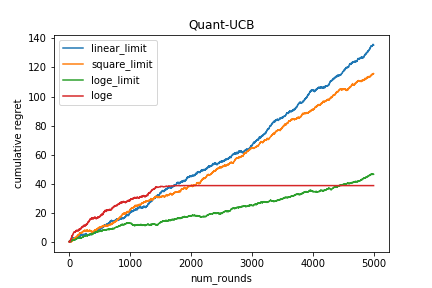
\includegraphics[scale=0.6]{Pictures/QuantUCB.png}
    		\label{QuantUCB}
    		\caption{QuantUCB (Discrete)}
    	\end{minipage}
    	\hspace{3cm}
    	\begin{minipage}[t]{0.4\textwidth}\centering   
    		\centering
    		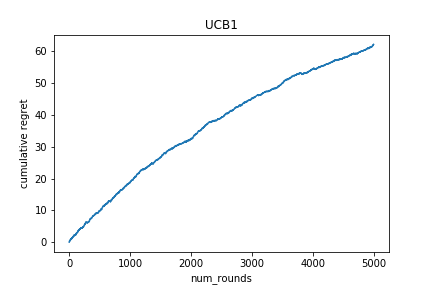
\includegraphics[scale=0.6]{Pictures/UCB1.png}
    		\label{UCB1}
    		\caption{UCB1}
    	\end{minipage}
    \end{figure}
    \item \href{https://github.com/chengsoonong/eheye/blob/master/QuantUCB/QuantUCB(continuous) with skewed noise.ipynb}{Continuous QuantUCB}\\
    Compared with GPUCB.
    
    \item Others\\
    \href{https://github.com/chengsoonong/eheye/blob/master/QuantUCB/How quantile changes when meeting more data.ipynb}{How quantile changes when meeting more data}\\
    \href{https://github.com/chengsoonong/eheye/blob/master/QuantUCB/Estimation evaluation.ipynb}{Comparison of skewed distribution estimation.}
\end{enumerate}
    
\item Open questions
    \begin{itemize}
        \item Does cumulative regret bounds exist for Quant-UCB? If so, how to prove the regret bound theoretically? 
        \item Compared with GP-UCB, what advantages and disadvantages does Quant-UCB have? In other words, under what constraints or for what kind of data, Quant-UCB performs better?
        \item What optimization algorithm we should use for Quant-UCB? For example, one choice could be making use of stochastic sub-gradient descent (SSGD) to perform sequential optimization; another possibility is to use dual optimization for joint quantile regression, as proposed in \cite{Sangnier:2016:JQR:3157382.3157511}.
        \item How to measure the performance of the proposed algorithm? i.e. how do we know Quant-UCB can beat related algorithms under some certain constraints? By measuring cumulative regret? efficiency? 
    \end{itemize}
    
\item Some considerations:



\end{enumerate}





\printbibliography

\end{document}
\grid
\grid